%\documentclass[12pt,t]{beamer}
\documentclass[xcolor=svgnames]{beamer}

%\usecolortheme[named=DarkBlue]{structure}

\usetheme{Boadilla}
%\usetheme[heigth=7mm]{Rochester}
%\usetheme{Rochester}
%\usetheme{Warsaw}
\usecolortheme{whale}
\useoutertheme{infolines}

\setbeamertemplate{blocks}[rounded][shadow=true]
%\setbeamertemplate{navigation symbols}{}
\usepackage[english]{babel}
\usepackage[utf8]{inputenc}
\usepackage{graphicx}
\usepackage{subfigure} 					% uso de many figures


\usepackage{color}
%\usepackage[usenames,dvipsnames,svgnames,table]{xcolor}
\usepackage{xcolor}
\usepackage{comment}
%\usepackage{algorithm2e}
\usepackage{algorithm}
\usepackage{algorithmic}
\usepackage{float}

%\floatname{algorithm}{Procedure}
\renewcommand{\algorithmicrequire}{\textbf{ \colorbox{yellow}{Input:} }}
\renewcommand{\algorithmicensure}{\textbf{  \colorbox{yellow}{Output:} } }
 \definecolor{keywordColor}{RGB}{165, 42, 42}
 \definecolor{componentColor}{RGB}{0, 0, 205}

\renewcommand{\algorithmicfor}{\textcolor[RGB]{165, 42, 42}{\textbf{For}}}
\renewcommand{\algorithmicendfor}{\textcolor[RGB]{165, 42, 42}{\textbf{End}}}
\renewcommand{\algorithmicdo}{\textcolor[RGB]{165, 42, 42}{\textbf{Do}}}
\renewcommand{\algorithmicreturn}{\textcolor[RGB]{165, 42, 42}{\textbf{Return}}}


\bibliographystyle{apalike}
% ------numbering frames-----------------------------------------%
%\newcommand*\oldmacro{}%
%\let\oldmacro\insertshorttitle%
%\renewcommand*\insertshorttitle{%
%	  \oldmacro\hfill%
%	  \insertframenumber\,/\,\inserttotalframenumber
%}
% ---------------------------------------------------------------%

% ------ References ---------------------------------------------%
\usepackage[absolute,overlay]{textpos}
\newenvironment{reference}[2]{%
  \begin{textblock*}{\textwidth}(#1,#2)
      \footnotesize\it\bgroup\color{red!50!black}}{\egroup\end{textblock*}}
% ---------------------------------------------------------------%

%\renewcommand{\figurename}{Figura}
%\renewcommand{\tablename}{Tabela}

% -------------------------------------------------------------- %
% Pacote necessario para subfiguras
\usepackage{multimedia, multirow}
\graphicspath{{./figures/}}
% -------------------------------------------------------------- %



\title[IEEE CAMAD 2012]
    {A Methodology to Define QoS and SLA Requirements in Service Choreographies}
\author[Alfonso Phocco-Diaz]
	{
		{\bf Authors} \\
		Victoriano Alfonso Phocco Diaz \\%\footnote{O aluno recebeu apoio financeiro do CNPq, processo 133147/2009-6} \\ [1ex]
		Daniel Macedo Batista
		%{\bf Orientador} \\  Daniel Macedo Batista 	\\
		%%{\bf Co-orientador} \\  Marco Dimas Gubitoso 	
	}
\institute[IME-USP]
	{Institute of Mathematics and Statistics \\
	 Departament of Computer Science \\	
	 University of Sao Paulo  \\  [1ex]
	 \texttt{alfonso7@ime.usp.br, batista@ime.usp.br}
	}
\date[September 2012]{September 17, 2012}



%%% Slides ---------------------------------
\begin{document}
%\pgfdeclareimage[width=180pt,height=20pt]{test}{images/header.jpg}
%\logo{\pgfuseimage{test}}


% --- the titlepage frame ------------------------------------------%
\begin{frame}[plain]
  \titlepage
\end{frame}


\section*{Agenda}
    \begin{frame}{Agenda}
        \tableofcontents
    \end{frame}

% ------------------------------------------------------------------%
\AtBeginSection[]
{
	\begin{frame}<beamer>
		\frametitle{}
		\tableofcontents[currentsection]
	\end{frame}
}

% ------------------------------------------------------------------%
% ------------------------------------------------------------------%
% --- Basic Concepts ---------------------------------------------------%
\section{Introduction}
  
% -----  SOC ----------%
    \begin{frame}{SOC}
       	\begin{block}{SOC (Service Oriented Computing)}\vspace{-.3\baselineskip}
          It  is a new computing paradigm that utilizes services as the basic constructs to support the development
	  of rapid, low-cost and easy composition of distributed applications even in
	  heterogeneous environments.  [Papazoglou et al., 2006]. %\cite{Papazoglou2007}.
        \end{block}
        Key elements:

        \begin{itemize}
           \item <1-> \colorbox{yellow}{Services} (mainly Web services).
           \item <2-> \colorbox{yellow}{SOA}.
           \item <3-> \colorbox{yellow}{Service Composition}.
	    \begin{itemize}
                  \item <4-> \colorbox{yellow}{\textbf{Service Orchestration}}.
                  \item <5-> \colorbox{yellow}{\textbf{Service Choreography}}.
                \end{itemize}
           \item <6->...
        \end{itemize}

    \end{frame}


%----------------- SOA -------------------%
  \begin{frame}{Web Services and SOA}
    	         \only<1>{	
              \begin{figure}[!h]
                  \centering
                  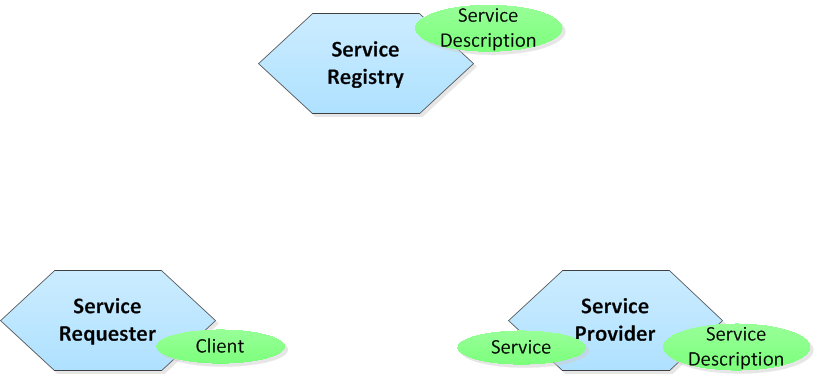
\includegraphics[width=0.9\textwidth]{SOA-Triangle_1.png}
                  \caption{SOA triangle (based on [W3C, 2002])}
              \end{figure}	
          }
          \only<2>{	
              \begin{figure}[!h]
                  \centering
                  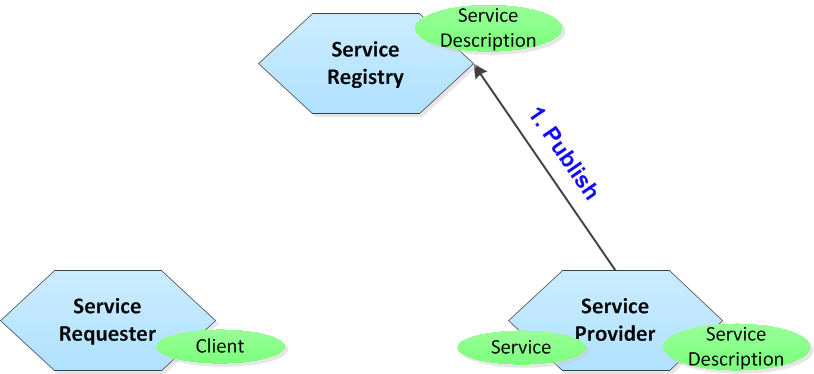
\includegraphics[width=0.9\textwidth]{SOA-Triangle_2.png}
                  \caption{SOA triangle (based on [W3C, 2002])}
              \end{figure}	
          }
          \only<3>{	
              \begin{figure}[!h]
                  \centering
                  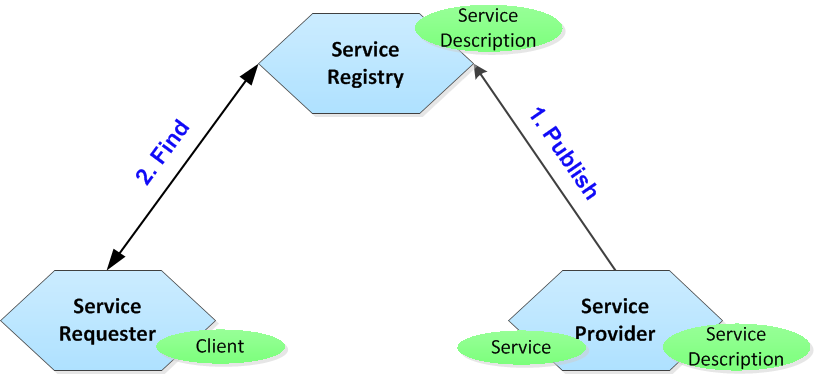
\includegraphics[width=0.9\textwidth]{SOA-Triangle_3.png}
                  \caption{SOA triangle (based on [W3C, 2002])}
              \end{figure}	
          }

          \only<4>{	
              \begin{figure}[!h]
                  \centering
                  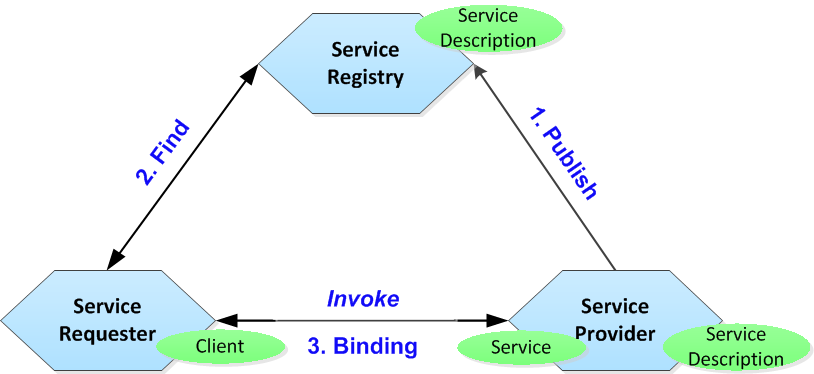
\includegraphics[width=0.9\textwidth]{SOA-Triangle_4.png}
                  \caption{SOA triangle (based on [W3C, 2002])}
              \end{figure}	
          }
          \only<5>{	
              \begin{figure}[!h]
                  \centering
                  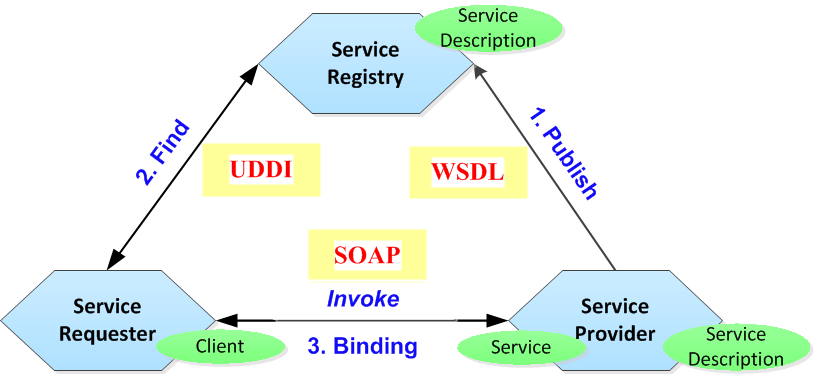
\includegraphics[width=0.9\textwidth]{SOA-Triangle_5.png}
                  \caption{SOA triangle (based on [W3C, 2002])}
              \end{figure}	
          }

    \end{frame}


    %----- Service Orchestration -----%
    \begin{frame}{Service Orchestration}
          \only<1>{	
              \begin{figure}[!h]
                  \centering
                  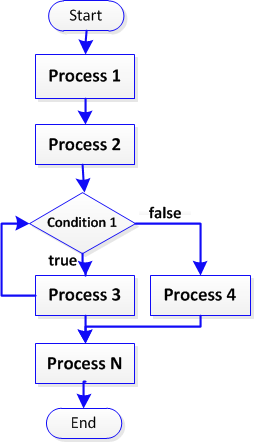
\includegraphics[width=0.25\textwidth]{Orchestration_1.png}
                  \caption{Service Orchestration}
              \end{figure}	
          }
          \only<2>{	
              \begin{figure}[!h]
                  \centering
                  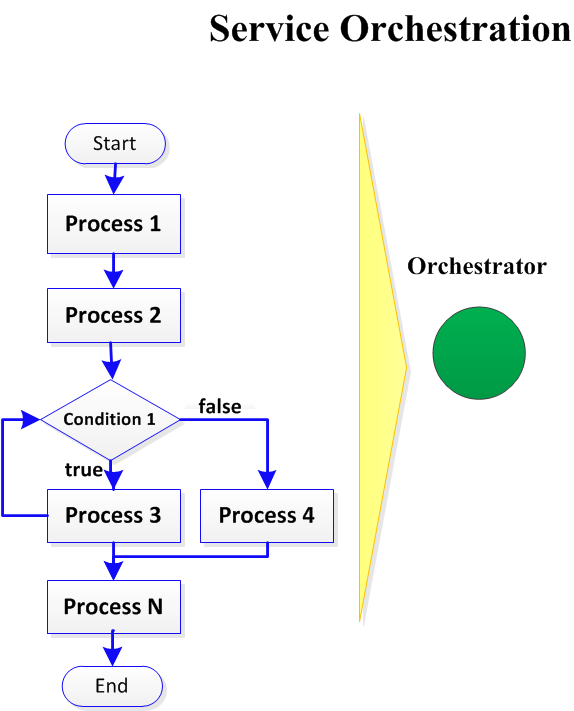
\includegraphics[width=0.45\textwidth]{Orchestration_2.png}
                  \caption{Service Orchestration}
              \end{figure}	
          }
          \only<3>{	
              \begin{figure}[!h]
                  \centering
                  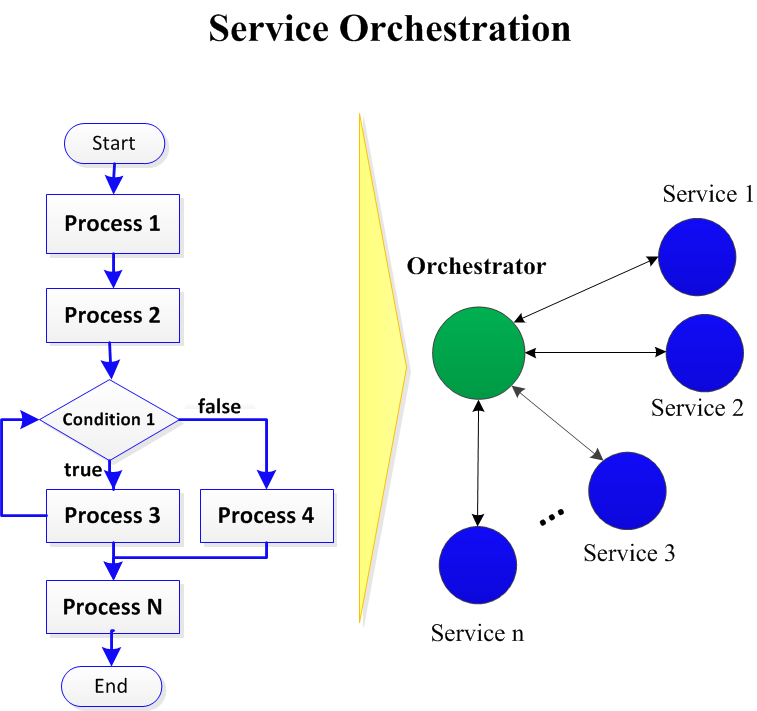
\includegraphics[width=0.5\textwidth]{Orchestration_3.png}
                  \caption{Service Orchestration}
              \end{figure}	
          }

  \end{frame}


    %----- Service Choreography -----%
    \begin{frame}{Service Choreography}
          \only<1>{
	      \begin{itemize}
	        \item Allows service composition in a \textbf{collaborative} manner.
		\item Describes the \textbf{P2P interactions} of the externally \textbf{observable behavior of its participants}.
		\item Don’t have a single point of control or coordination.
	      \end{itemize}

	      
              \begin{figure}[!h]
                  \centering
                  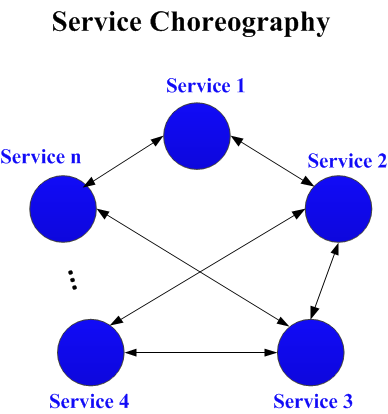
\includegraphics[width=0.4\textwidth]{ChoreographyA.png}
                  \caption{Service Choreography}
              \end{figure}	
          }
          %\only<2>{	
           %   \begin{figure}[!h]
            %      \centering
            %      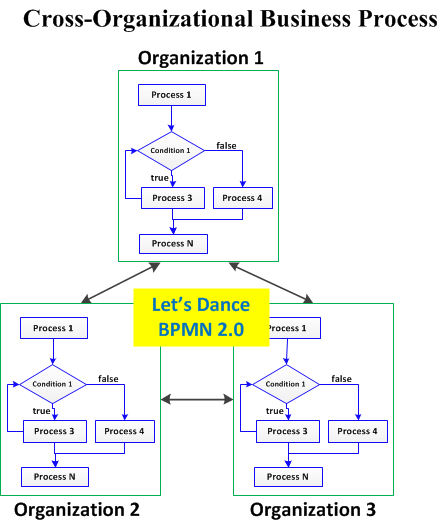
\includegraphics[width=0.6\textwidth]{ChoreographyB_1.png}
            %      \caption{Service Choreography}
            %  \end{figure}	
          %}
          \only<2>{	
              \begin{figure}[!h]
                  \centering
                  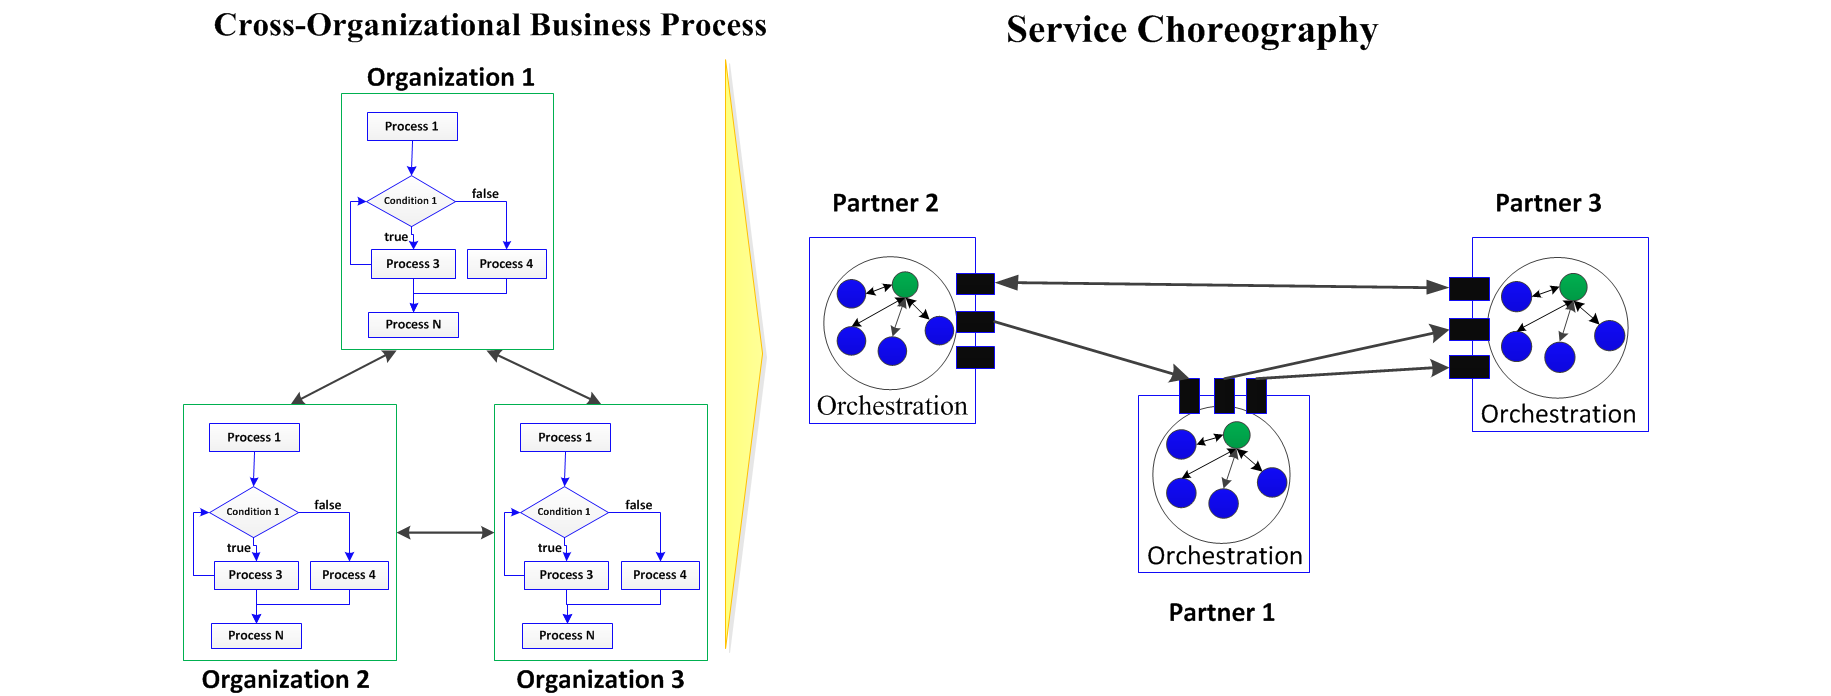
\includegraphics[width=1.0\textwidth]{ChoreographyB_2.png}
                  \caption{Service Choreography}
              \end{figure}	
          }
          \only<3>{	
              \begin{figure}[!h]
                  \centering
                  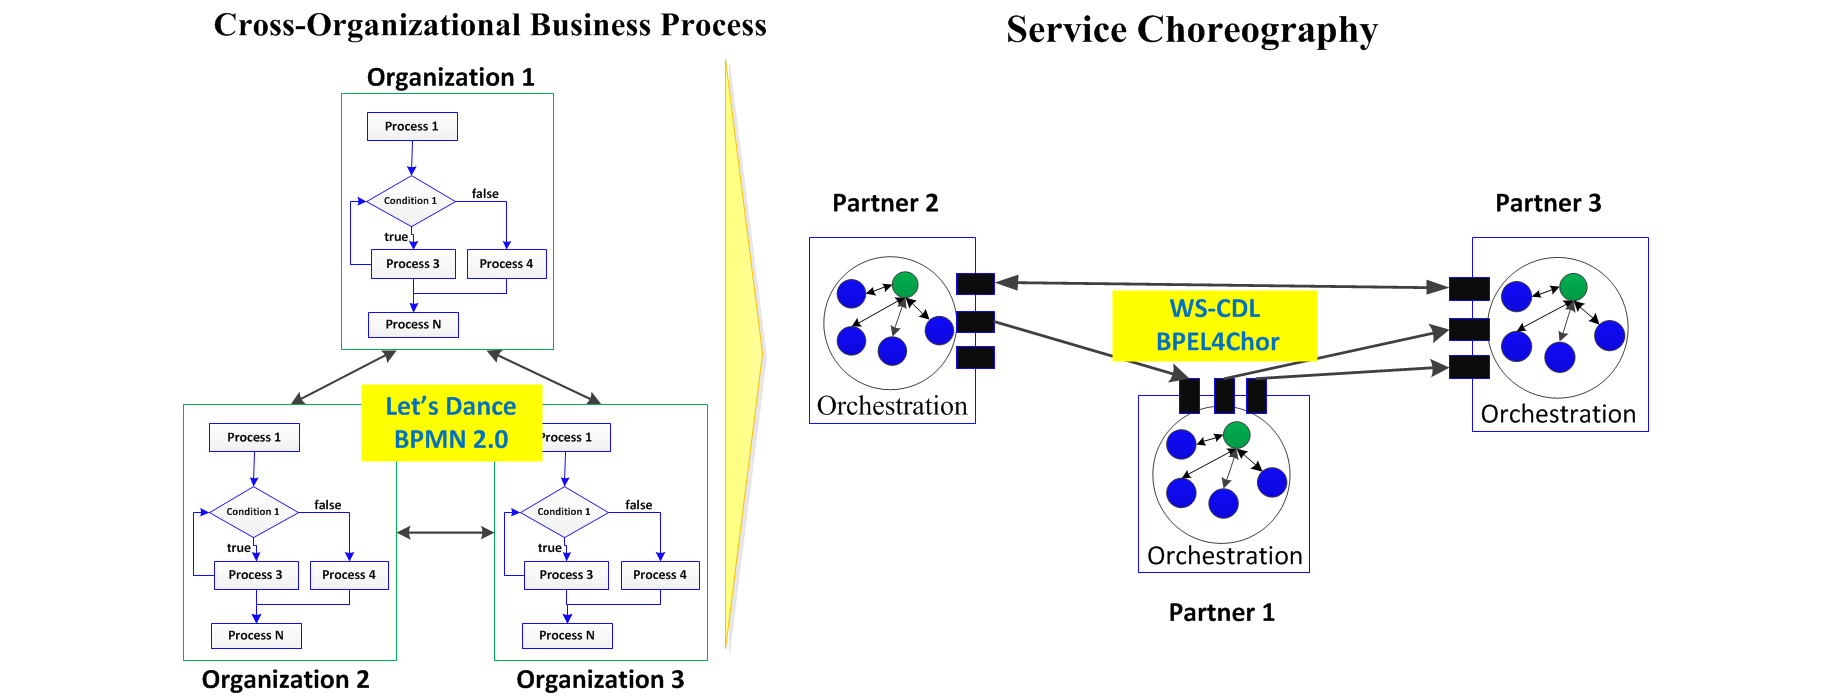
\includegraphics[width=1.0\textwidth]{ChoreographyB_3.png}
                  \caption{Service Choreography}
              \end{figure}	
          }
    \end{frame}

%----- QoS -----
%\begin{frame}{Quality of service}



  \begin{frame}{BPMN and Choreography}
    \begin{itemize}
      \item <1-> A Choreography is a type of process.
	\begin{itemize}
	  \item Differs in purpose and behavior from a standard BPMN Process (Process Orchestration). 
	  \item Formalizes the way business \colorbox{yellow}{Participants} \textbf{coordinate} their \colorbox{yellow}{interactions}.
	\end{itemize}
      \item <2-> Focus on the exchange of information (\colorbox{yellow}{Messages}) between these Participants.
      \item <3-> Two approaches:
	\begin{itemize}
	  \item <4-> \colorbox{yellow}{Interconnection Model}: With collaborations diagrams. 
	  \item <5-> \colorbox{yellow}{Interaction Model}:  BPMN Choreographies. using special activities (\textit{Choreography Activity}). 
	\end{itemize}
    \end{itemize}
    
  \end{frame}


  \begin{frame}{Interconnection Model}
      \begin{itemize}
	\item Interconnected public views.	
	\item Use of standard activities.
 	\item ``Collaboration'' in BPMN 2.0.
      \end{itemize}
   \begin{figure}[!h]
	    \centering
	    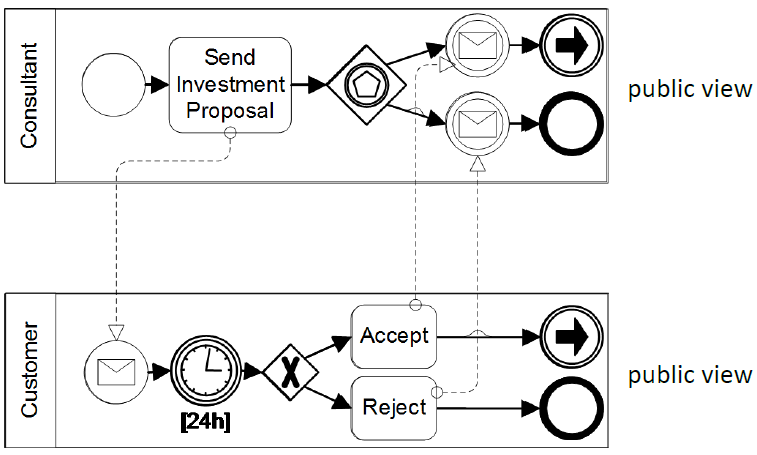
\includegraphics[width=0.8\textwidth]{interconnection_choreography.png}
	    %\caption{BPMN elements for modeling choreographies.}
    \end{figure}	 
  \end{frame}


  \begin{frame}{Interaction Model}
    \begin{itemize}
	  \item Interactions \textbf{globally captured}.	
	  \item Basic building block: \textbf{atomic interaction} between two parties.
	  \item ``Choreography'' in BPMN 2.0.
	\end{itemize}
    \begin{figure}[!h]
	      \centering
	      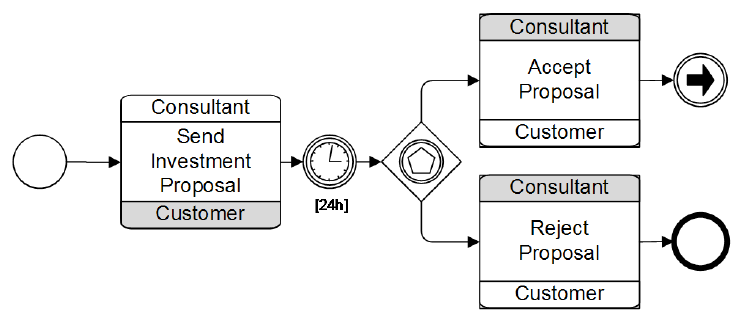
\includegraphics[width=0.8\textwidth]{interaction_choreography.png}
	      %\caption{BPMN elements for modeling choreographies.}
      \end{figure}	 
  \end{frame}


  \begin{frame}{BPMN Choreography}
    
    \begin{figure}[!h]
	      \centering
	      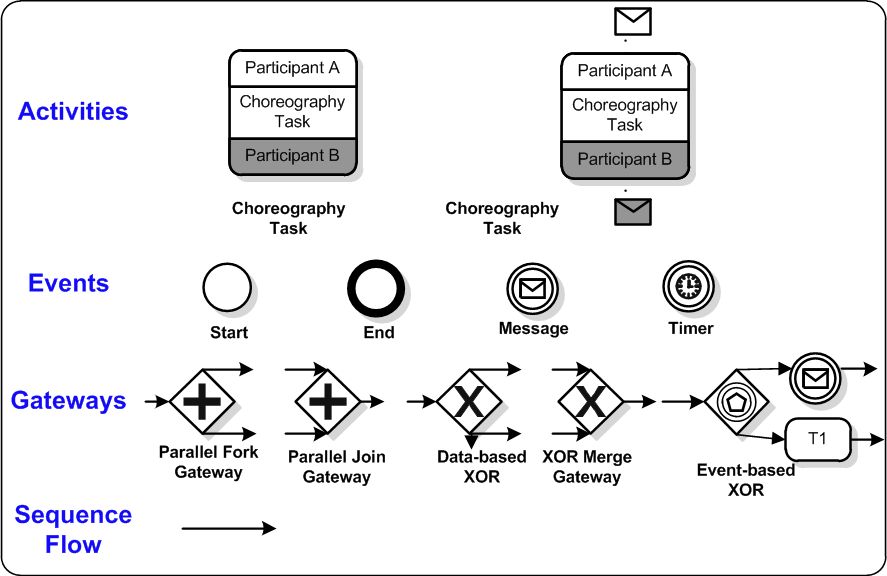
\includegraphics[width=0.8\textwidth]{BPMNBasicChoroegraphy.png}
	      \caption{BPMN elements for modeling choreographies (BPMN 2.0).}
      \end{figure}	 
  \end{frame}
  
  \begin{frame}{ Generalized Stochastic Petri Net (GSPN) (I)}
   
  \end{frame}

  \begin{frame}{ Generalized Stochastic Petri Net (GSPN) (II)}
   
  \end{frame}
% ------------------------------------------------------------------%
% ------------------------------------------------------------------%
% ------ Problem ---------------------------------------------------%
\section{Problem}


    \begin{frame}{Problem to Solve}
    	\begin{itemize}
          \item <1-> Planning of resources before/during development of choreography.
          \item <2-> Little approaches don't evaluate choreographies:
	    \begin{itemize}
	      \item focusing on \textbf{QoS} or
	      \item in earlier stages of development.
	    \end{itemize}
          \item <3-> To guarantee QoS about communications (network) is important. 
    	\end{itemize}
    \end{frame}

    \begin{frame}
        \begin{block}{Objectives }\vspace{-.3\baselineskip}
        	\begin{itemize}
                  \item To assess the \textbf{impact of QoS} attributes in a \textbf{choreography interaction model}.
		  \item To propose a novel methodology to establish \textbf{requirements for QoS and SLA} in \textbf{early stages of development}.
		  \item To plan the capacity of the network elements in choreographies.
		  \item To convert a interaction model to a GSPN (Generalized Stochastic Petri Net) with QoS.
            \end{itemize}
        \end{block}
    \end{frame}

    
\begin{comment}
  \begin{frame}{Justification}
    	\begin{itemize}
          \item <1-> Planning of resources before/during development of choreography.
          \item <2->\textbf{QoS} is a important factor for adaptation, selection, optimization, service composition into SOC.
          plan the capacity of the network elements connecting
the hosts involved in the enactment and deployment of the
choreography.
    	\end{itemize}
  \end{frame}

\end{comment}

% ------------------------------------------------------------------%
% ------------------------------------------------------------------%
% -------------------- Methodology ---------------------------------%
\section{Methodology}
  \begin{frame}{Description}
    \begin{enumerate}
      \item <1-> Mapping of a choreography to a GSPN.
	  \begin{itemize}
	    \item The choreography is specified according ``interaction model''.
	    \item The choreography is specified in BPMN 2.0.
	    \item The resulting GSPN include a QoS model.
	  \end{itemize}

      \item <2-> Configurations of resulting GSPN. 
      \item <3-> Simulations of scenarios.
    \end{enumerate}

  \end{frame}


  \begin{frame}{Choreography Formalization}
    \begin{block}{ Definition: Process Choreography }\vspace{-.3\baselineskip}
      A process choreography  is a tuple: 
            \textbf{ $PC = (\mathcal{O, A, E, G, T}, \{e^S\}, \mathcal{E}^I, \{e^E\}, \mathcal{E}^{I_M}, \mathcal{E}^{I_T}, \mathcal{G}^F, \mathcal{G}^J,$
       $\mathcal{G}^X, \mathcal{G}^M, \mathcal{G}^V, \mathcal{F} )$} where:
      
      \begin{itemize}
	  \item \textbf{$\mathcal{O}$} is a set of objects and it's partitioned in \textbf{activities $\mathcal{A}$}, \textbf{events $\mathcal{E}$} and \textbf{gateways $\mathcal{G}$}.
	  \item \textbf{$\mathcal{A}$}, is the set of \textbf{choreography tasks $\mathcal{T}$}.
	  \item \textbf{$\mathcal{E}$} is the set of \textbf{events} and  it's is partitioned in \textbf{Start event {$e^\mathcal{S}$}}, \textbf{Intermediate
	events $\mathcal{E^I}$} and \textbf{End event {$e^\mathcal{E}$}}.
	  \item \textbf{$\mathcal{G}$} é the set of \textbf{gateways} and is partitioned in \textbf{parallel fork gateways $\mathcal{G}^F$},
	\textbf{parallel join gateways $\mathcal{G}^J$}, \textbf{data-based XOR gateways $\mathcal{G}^X$}, \textbf{XOR merge gateways $\mathcal{G}^V$} and \textbf{event-based
	XOR gateways $\mathcal{G}^M$}.
	\item \textbf{$\mathcal{F} \subseteq \mathcal{O}x\mathcal{O}$} is the control flow relation, i.e. a \textbf{set of sequence flows connecting objects}.
      \end{itemize}
      
    \end{block}

  \end{frame}

  
  \begin{frame}{QoS Model}
    \begin{itemize} %%Perhaps it's needed use some picture, for example life cycle call service. 
	\item Defining the QoS attributes involved in \textbf{service}, \textbf{network} and \textbf{message} aspects.
	\item QoS attributes:
	    \begin{itemize}
	      \item In service operation: time to complete the service.
	      \item In network: delay and communication errors. 
	      \item In message: format of message.
	    \end{itemize}
    \end{itemize}
  \end{frame}


  \begin{frame}{Mapping BPMN to Petri Net (I)}
    \begin{figure}[!h]
      \centering
      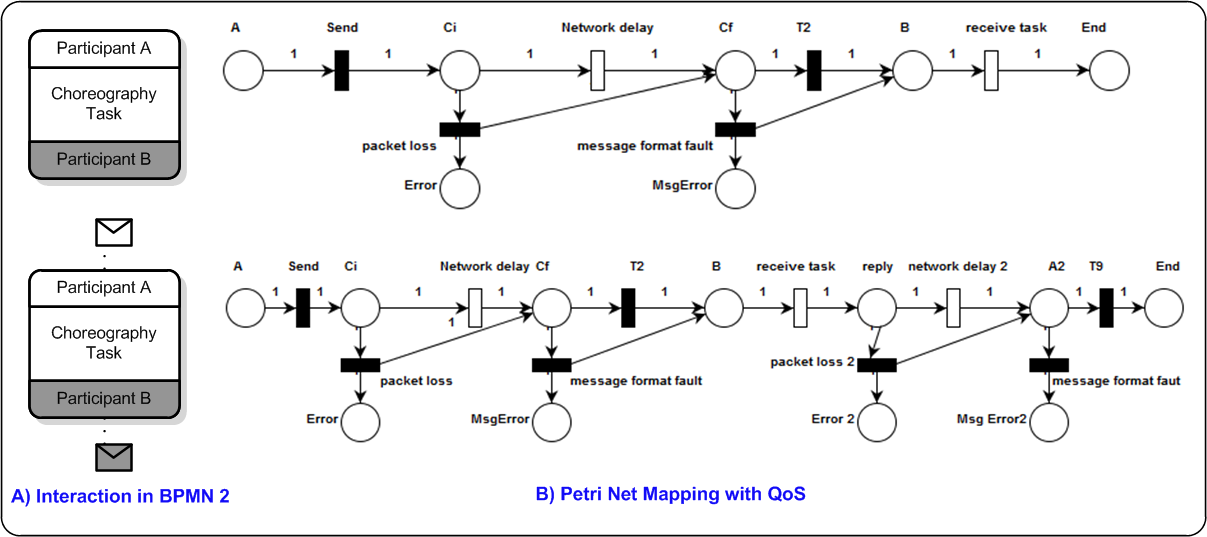
\includegraphics[width=0.8\textwidth]{BPMNChoreographies1-QoS1.png}
      \caption{  Mapping of two different choreography tasks with the QoS model}      
    \end{figure}   
  \end{frame}


  \begin{frame}{Mapping BPMN to Petri Net (II)}
    \begin{figure}[!h]
	\centering
	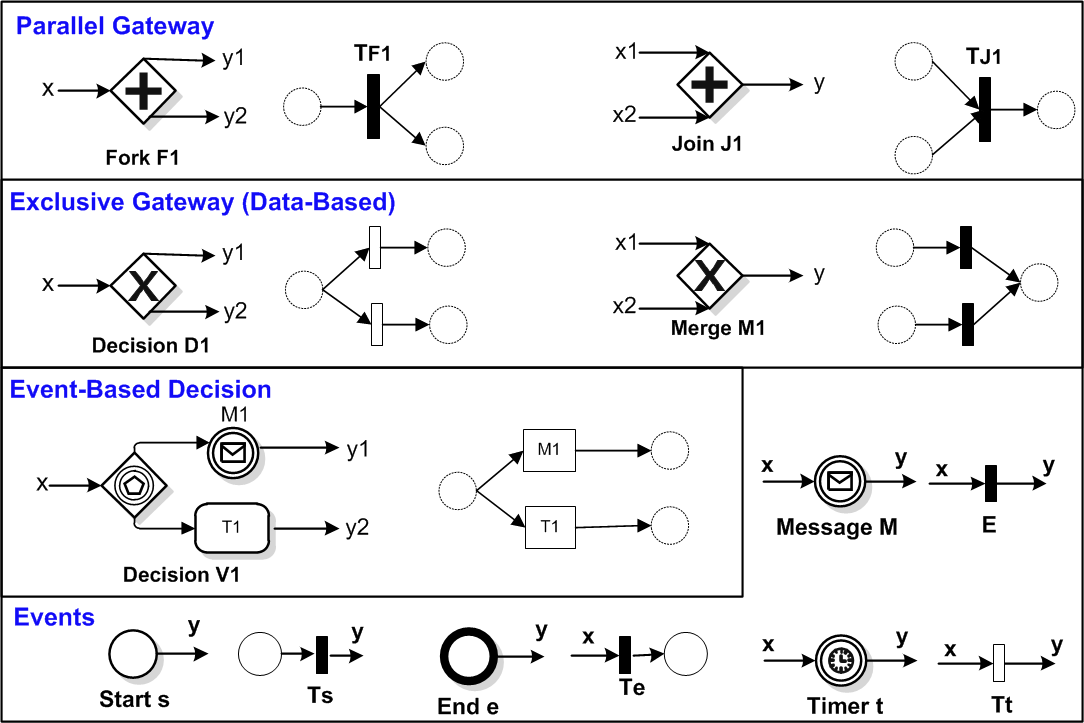
\includegraphics[width=0.8\textwidth]{BPMNChoreographies2_2.png}
	\caption{Mapping of events and gateways elements to modules of Petri nets}
     \end{figure}   
  \end{frame}

  
  \begin{frame}{Mapping Algorithm (I)}
      \begin{algorithm}[H]
	  %\caption{Mapping a Interconnection Choreography in BPMN onto a GSPN with QoS model}
	    %\caption{ { \small Mapeamento de uma coreografia especificada em BPMN 2.0 para uma GSPN com o modelo de QoS } }
	    \caption{ { \footnotesize Mapping of choreography specified in BPMN 2.0 to a GSPN with QoS model} }
	    %\label{alg2}
	    \begin{algorithmic}
	    { \footnotesize
	      %\REQUIRE Process Choreography $\mathcal{PC}$ in BPMN 2.0.
	      \uncover<0->{ \REQUIRE \textbf{Process Choreography} \textcolor{componentColor}{ \textbf{ $PC = (\mathcal{O, A, E, G, T}, \{e^S\}, \mathcal{E}^I,$ $\{e^E\}, \mathcal{E}^{I_M}, \mathcal{E}^{I_T}, 
	      \mathcal{G}^F, \mathcal{G}^J,$ $\mathcal{G}^X, \mathcal{G}^M, \mathcal{G}^V, \mathcal{F} )$} } in BPMN 2.0. }

	      \uncover<1->{ \ENSURE Generalized Stochastic Petri Net \textcolor{componentColor}{ \textbf{$GSPN_{QoS}$} }.  }
	      
	    \vspace*{3 mm}
	     \uncover<2->{ \STATE Consider \textcolor{componentColor}{ \textbf{$CT_i \in \mathcal{T} $, $G_j \in \mathcal{G} $}} and \textcolor{componentColor}{ \textbf{$E_k \in \mathcal{E}$}. where  $i, j, k \in \mathbb{N} $}. }
	      %\STATE Let $PNQoS(CT_i)$ a respective GSPN including QoS from type of $CT_i$ and according to mapping rules (Figure \ref{fig:MappingTaskChoreographiesQoS1}).
	      %\STATE Let $PNQoS(CT_i)$ be a respective GSPN including QoS from type $CT_i$ and according to mapping rules (Figure \ref{fig:MappingTaskChoreographiesQoS1}).
	    \vspace*{3 mm}
	      \uncover<3->{ \STATE Consider \textcolor{componentColor}{ $PNQoS(CT_i)$ } is a function of the type of \textcolor{componentColor}{ $CT_i$} that returns a GSPN according to mapping rules. }
	     \uncover<4->{ \STATE Consider \textcolor{componentColor}{ $PNQoS(G_j)$ } is a function of the type of \textcolor{componentColor}{$G_j$ } that returns a GSPN according to mapping rules. }
	     \uncover<5->{ \STATE Consider \textcolor{componentColor}{ $PNQoS(E_k)$ } is a function of the type of \textcolor{componentColor}{$E_k$} that returns a GSPN according to mapping rules. }
	    \vspace*{3 mm}
	     \uncover<6->{ \STATE Consider \textcolor{componentColor}{ \textbf{$\oplus$} } the binary operator of composition of two GSPNs that returns other GSPN. }

	    }
	\end{algorithmic}
 
      \end{algorithm}

  \end{frame}


%165,42,42
  \begin{frame}{ Mapping Algorithm (II)}
       

    \begin{algorithm}[H]
%	    \caption{ { \small Mapping of choreography specified in BPMN 2.0 to a GSPN with QoS model} }
%	    \label{alg2}
	    \begin{algorithmic}
	    { \footnotesize
	      
	      \uncover<1->{  \STATE $\textcolor{componentColor}{GSPN_{QoS} } \leftarrow  Empty\  Petri\  Net$  }

	      %\FOR { $CT_i \in T $ }
	      % \STATE $GSPN_{QoS} \leftarrow GSPN_{QoS} \oplus PNQoS(CT_i)$
	      %\ENDFOR

	      \uncover<2->{   \FOR { $\textcolor{componentColor}{ CT_i} \in \textcolor{componentColor}{\mathcal{T}} $ } }  
		\uncover<3->{ \STATE $\textcolor{componentColor}{ GSPN_{QoS} } \leftarrow \textcolor{componentColor}{ GSPN_{QoS} } \oplus \textcolor{componentColor}{ PNQoS(CT_i) } $  		}
		\uncover<4->{ \STATE Add a arrival \textbf{timed Transition} at beginning of the \textcolor{componentColor}{$GSPN_{QoS}$}.   }
	     \uncover<2->{  \ENDFOR }
	      \vspace*{3 mm}
	      \uncover<5->{ \FOR{ $\textcolor{componentColor}{G_j} \in \textcolor{componentColor}{\mathcal{G}} $ } 			}
		\uncover<6->{	\STATE $\textcolor{componentColor}{ GSPN_{QoS} } \leftarrow \textcolor{componentColor}{GSPN_{QoS}} \oplus \textcolor{componentColor}{ PN(G_j) }$	}
	      \uncover<5->{ \ENDFOR	}
	    \vspace*{3 mm}
	    \uncover<7->{ \FOR{ $\textcolor{componentColor}{ E_k } \in \textcolor{componentColor}{ \mathcal{E} } $ }					}	
		\uncover<8->{ \STATE $\textcolor{componentColor}{ GSPN_{QoS} } \leftarrow \textcolor{componentColor}{ GSPN_{QoS} } \oplus \textcolor{componentColor}{ PN(E_k) }$  	}
	      \uncover<7->{ \ENDFOR		}
	      \vspace*{3 mm}
	      \uncover<9->{ \STATE Add a starting Place and \textbf{immediate Transition} at the beginning of the \textcolor{componentColor}{ $GSPN_{QoS}$}.	}
	      \uncover<10->{ \STATE Add a ending Place and \textbf{immediate Transition} at the end of the \textcolor{componentColor}{$GSPN_{QoS}$}.	}
	      \vspace*{3 mm}
	      \uncover<11->{ \RETURN \textcolor{componentColor}{$GSPN_{QoS}$}		}
	    }
	\end{algorithmic}
 
      \end{algorithm}
  \end{frame}

  


  

% ------------------------------------------------------------------%
% ------------------------------------------------------------------%
% -------------------- Performance Evaluation ----------------------%
\section{Performance Evaluation}
  \begin{frame}{Scenario}
  
  \end{frame}


  \begin{frame}{Mapping}
   
  \end{frame}


  \begin{frame}{ Configuration}
   
  \end{frame}


  \begin{frame}{ Simulation}
   
  \end{frame}



  \begin{frame}{ Results}
   
  \end{frame}





%---------- Conclusions ----------------
\section{Conclusions and Future Works}
   \begin{frame}{Conclusions}
       \begin{itemize}
         \item <1->  We have prosposed a Nobel methodology to aid define QoS and SLA requirements in service Choreography.
	 \item <2->  
       \end{itemize}
   \end{frame}

  \begin{frame}{Future Works}
       \begin{itemize}
         \item <1->  .
	 \item <2->  
       \end{itemize}
   \end{frame}



%\bibliographystyle{apalike}% 
%\def\newblock{}
 %       \bibliography{slides}
 %   \end{thebibliography}
%\end{frame}


%--------- fim ----------
    \begin{frame}%{\textbf{Thanks!}}
        \begin{block}{}\vspace{-.3\baselineskip}
        	Thanks so much!
        \end{block}

    \end{frame}




\end{document}